\documentclass[conference]{IEEEtran}
\usepackage{graphicx}
\usepackage[noadjust]{cite}
\usepackage[acronym]{glossaries} 
\makeglossaries

\begin{document}
\newacronym{ipv4}{IPv4}{Internet Protocol Version 4}
\newacronym{ipv6}{IPv6}{Internet Protocol Version 6}
\newacronym{iot}{IoT}{Internet of Things}
\newacronym{j2se}{J2SE}{Java Standard Edition}
\newacronym{tinyos}{TinyOS}{TinyOS}
\newacronym{nesc}{NesC}{NesC}
\newacronym{http}{HTTP}{Hypertext Transfer protocol}
\newacronym{sg}{SG}{Smart Grid}
\newacronym{wsn}{WSN}{Wireless Sensor Network}
\newacronym{rfid}{RFID}{Radio Frequency Identification}
\newacronym{dr}{DR}{Demand Response}
\newacronym{6lowpan}{6LoWPAN}{IPv6 over Low power Wireless Personal Area Networks}
\newacronym{ip}{IP}{Internet Protocol}
\newacronym{tcp}{TCP}{Transmission Control Protocol}
\newacronym{udp}{UDP}{User Datagram Protocol}
\newacronym{usb}{USB}{Universal Serial Bus}
\newacronym{res}{RES}{Renewable Energy Sources}
\newacronym{dg}{DG}{Distributed Generation}
\newacronym{ami}{AMI}{Advanced Metering Infrastructure}
\newacronym{m2m}{M2M}{Machine to Machine communications}
\newacronym{rdbms}{RDBMS}{Relational Database Management System}
\newacronym{osi}{OSI}{Open Systems Interconnection}
\newacronym{ct}{CT}{Current Transformer}
\newacronym{wh}{Wh}{Watt Hour}
\newacronym{a}{A}{Ampere}
\newacronym{w}{W}{Watt}
\newacronym{v}{V}{Volt}
\newacronym{blip}{BLIP}{Berkeley Low-power IP stack}
\newacronym{os}{OS}{Operating System}
\newacronym{ietf}{IETF}{Internet Engineering Task Force}
\newacronym{ims}{IMS}{IP Multimedia Subsystem}
\newacronym{owl}{OWL}{Web Ontology Language}
\newacronym{cps}{CPS}{Cyber Physical System}
\newacronym{gsm}{GSM}{Global System for Mobile Communications}
\newacronym{aodv}{AODV}{Ad hoc On-Demand Distance Vector}


\title{Towards the Internet of Things: A Real-World Test-bed}
\author{\IEEEauthorblockN{Nacer Khalil}
\IEEEauthorblockA{School of Electrical and Engineering\\
Al Akhawayn University In Ifrane\\
Email: n.khalil@aui.ma}
\and
\IEEEauthorblockN{Mohamed Riduan Abid}
\IEEEauthorblockA{School of Electrical and Engineering\\
Al Akhawayn University In Ifrane\\
Email: r.abid@aui.ma}
\and
\IEEEauthorblockN{Driss Benhaddou}
\IEEEauthorblockA{School of Engineering and Technology\\
University of Houston\\
Email: dbenhaddou@uh.edu}}
\maketitle
\begin{abstract}
The Internet is smoothly migrating from an Internet of people to an Internet of Things. By 2050, it is expected to have 50 billions “Things” connected to the Internet. 
However, such a migration induces a strong level of complexity when handling interoperability between the heterogeneous things, e.g., Wireless sensor networks, \gls{rfid}\glsreset{rfid}, and mobile computing. In this context, a couple of standards have been already set, and they are currently reached the mature stage, e.g., \gls{ipv6}\glsreset{ipv6}, \gls{6lowpan}\glsreset{6lowpan}, \gls{m2m}\glsreset{m2m}, and \gls{ims}\glsreset{ims}. In this paper, we focus on the integration of wireless sensor networks to the Internet. We shed further on the subtleties of such integration, and we deployed a real-world testbed where wireless sensors are used to control electrical appliances in a smart building. 
\end{abstract}

\begin{IEEEkeywords}
WSN, 6LoWPAN, TinyOS, IoT, Cyber Physical System
\end{IEEEkeywords}

\section{Introduction}
The \gls{iot} is the future of Internet. It is an Internet where \textit{Things} communicate by producing and consuming information. This makes these \textit{Things} more intelligent as they are able to provide services but at the same time use others. These physical devices are uniquely identified in the Internet by making use of technologies such as \gls{ipv6} and \gls{rfid}. There will be millions of devices in the Internet both producing and consuming information \cite{ref8}. To build the \gls{iot}, there are key points that should be added to the actual Internet to make all this possible. The first point is to make the TCP/IP protocol stack based on \gls{6lowpan} adopted by all physical devices and \glspl{wsn}. The identification of each \textit{Thing} is possible by using \gls{rfid} which is a low power identification chip that allows one to identify objects uniquely. The second point is to standardize the communication and \gls{m2m} is adopted for this purpose.

\
To make of these \textit{Things} \glspl{cps}, they must have three main functionalities: sensing, computation and communication.Sensing is made possible using \glspl{wsn} that provide a basis to sense the environment. In addition, each mote is equipped with processing power that provides the computation functionality. Finally, communication is made using \gls{ipv6} as a network technology.

\
In this paper, we create a small network where a \gls{m2m} is possible. This network can be part of what is known as Internet of things \cite{ref1}. The deployed tested  is composed of a \gls{wsn}, a middle-ware, and a mobile client for smart home energy monitoring and control where data is collected from the motes within the \gls{wsn} and communicated to the middle-ware. The mobile client is able to monitor and visualize this data and control appliances remotely. The contributions of this paper are:
\begin{itemize}
\item The system is developed in a heterogeneous system,and makes it transparent
\item The \gls{wsn} uses \gls{ipv6} over \gls{6lowpan} and is able to communicate in the Internet
\item The Two-Way communication is built in the system 
\end{itemize}
The Rest of the paper is organized as follows: Section II presents related work. In Section III, a review of \gls{iot} concepts and issues are presented. Section IV introduces \gls{6lowpan} standard. Section V describes the system architecture. In section VI, the deployment of the system is discussed in details and section VII presents the experiments conducted to measure the system's performance and the findings of the system.
 
\section{Literature review}
\gls{sg} is perceived as one of the key applications based on \gls{iot}. It uses different technologies such as Zigbee, \gls{6lowpan}, \gls{m2m} and \gls{ims} \cite{ref1}.  The need to introduce \gls{ipv6} within the wireless sensor networks is discussed as well as the existing approaches and issues related to introducing IPV6 on top of Zigbee. Such issues are fragmentation, frame size, addressing, and security issues \cite{ref2}. This paper introduces a real testbed that includes the whole TCP/IP protocol implemented by \gls{blip} that takes into consideration most of those issues and implements the two-way communication as needed by smart grids and measures the performance of such a system. In addition, El Kouche investigates on the widely used architectures and technologies and explains which architecture is the most suitable for a WSN within the \gls{iot} \cite{ref3}. \cite{ref4} discusses the requirement of an \gls{iot} gateway and propose an architecture for the system to be deployed in the gateway. A rather similar architecture to what is done in this paper is proposed by Yerra, Bharathi, Rajalakshmi and Desai \cite{ref7}. They use \gls{gsm} to communicate information whereas in our case, Internet is used for this purpose. 

\
Research discusses the benefits of replacing Zigbee by Wi-Fi as this last offers higher bandwidth, non-line transmission ability, large-scale data collection, and is highly cost-effective. Still, Zigbee has the exclusive advantage of consuming the least energy of existing communication technologies which is something required in \gls{sg} and \gls{iot}, especially for systems deployed in difficult-to-access environments \cite{ref11}. 

\
From the architectural point of view, integrating \glspl{sg} within \gls{iot} imposes the need to address heterogeneity. An \gls{iot} gateway system based on Zigbee and GPRS protocols helps partly in dealing with the heterogeneity problem and therefore enable the \glspl{wsn} communicate with the mobile telecommunication network \cite{ref11}. Another solution to the heterogeneity problem is proposed with a new, light-weight web service transport protocol called Lean Transport Protocol (LTP) that will allow transparent exchange of web service messages between all kinds of devices. This protocol is platform-independent, low-energy communication \cite{ref12}. Other researchers claim that the major source of heterogeneity arises from the fact that there are different types of WSN devices e.g. Micaz, Mica2, and Telosb that do not use the same standards. They propose to move the communication in \glspl{wsn} to "all-IP" as this would remove most of the heterogeneity. However, there are already deployed legacy \glspl{wsn} which makes the task is complicated. Fortunately, an architecture is sketched that is capable of converting all the \glspl{wsn}, new and legacy, to support IPv6 \cite{ref13}.

\section{Internet of things}
\gls{iot} is new concept based on the idea that there will more \textit{Things} than humans connected to the Internet. This means that machines will play a major role in the Internet. The \textit{Things} will be able to communicate autonomously without the need to interact with human beings. \glspl{wsn} will be included in most \textit{Things} and therefore the sensory data will make a significant portion of the information flowing in the Internet. Nowadays, humans are the major players in the Internet but this trend is changing as there are over 12.5 billion devices connected nowadays in the Internet \cite{ref14}. In \gls{iot}, \gls{m2m} will be the main communication standard between different \textit{Things}. \gls{m2m} is used in this project between the middle-ware and the \gls{wsn} when monitoring and controlling an appliance. 

\
Ubiquitous computing and pervasive computing are key paradigms in \gls{iot}. Physical objects will be able to communicate in the Internet by producing and consuming information \cite{ref9}. \gls{rfid} is a technology that identifies physical devices while consuming very little energy. Another important technological component is \gls{wsn} that gives the physical objects the ability to sense the environment and communicate such information. Mobile computing and cloud computing are important components as most of the storage and processing power will come from the cloud. 

\
\gls{iot} will have a major impact on the every day life of people as it will affect our lives inside and outside our homes. The physical devices will be able to communicate and consume different types of information. More and more applications based on \gls{iot} are now being developed. Ideas such as smart farming, smart transportation, smart homes, smart health, smart postal and smart refrigerators are only a small subset of a myriad of applications that will come to life with \gls{iot} \cite{ref15}. Smart grid is another key application that benefits from \gls{iot}. The US national intelligence listed the Internet of things as being on six disruptive civil technologies with potential impact on the US national power \cite{ref10}.
\section{6LoWPAN}
\gls{6lowpan} stands for  "IPv6 over Low power Wireless Personal Area Networks". It stands for the name of the working group within the \gls{ietf}. It is based on the idea that all the \textit{Things} should be able to have the TCP/IP protocol stack and join the \gls{iot}. In order to be able to build the TCP/IP protocol stack in all devices, there have been multiple aspects of IP that have been modified. the IP maximum transmission unit(MTU) is fixed at 1280 Bytes, but the Zigbee MTU is only 127 Bytes. This means that not every \gls{ipv6} packets can be encapsulated within the Zigbee frame, and such issue has been addressed by \gls{6lowpan}. Another issue is related to the addressing with the 128 bits address; In \gls{6lowpan}, addressing via the \gls{ipv6} is performed hierarchically. The main purpose behind is to  identify the packet's destination network Id before forwarding it to the network. These were just two of a large set of issues that \gls{6lowpan} solves in order to enable even the low-power devices to join \gls{iot}. \gls{tinyos} as being one of the most used operating system in \glspl{wsn} comes with an implementation of \gls{6lowpan} through \gls{blip} that provides a lightweight implementation of the \gls{6lowpan}. This project makes use of \gls{blip} to provide the TCP/IP protocol stack to the \gls{wsn}.

\section{System Deployment}
The system is composed of four building blocks. 
\begin{itemize}
\item Wireless Sensor Network (WSN)
\item Gateway Server
\item Middle-ware
\item Mobile Client
\end{itemize}
The WSN uses Zigbee as the communication medium and uses \gls{ipv6} in the network layer. However, the communication between the gateway server, the middle-ware and the mobile client is done via Wi-Fi and \gls{ipv4} technology. This architecture enables any device within the system to communicate with any other device independently of the communication medium used (Zigbee or Wi-Fi) or the network technology used (\gls{ipv4} or \gls{ipv6}). Figure 1 is a network diagram that depicts the different components of the system as well as the interconnections that exist between the different components of the system.

\begin{figure}[htbp]
\centering
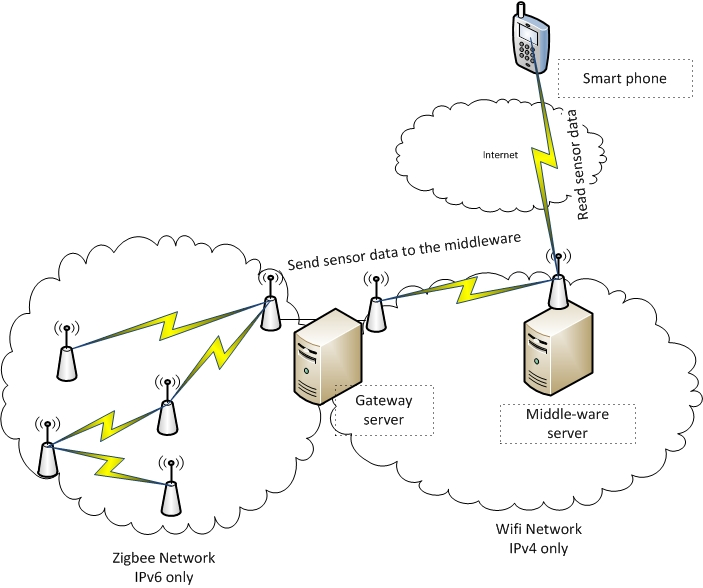
\includegraphics[scale=0.48]{images/network_diagram.jpg}
\caption{Network diagram}
\label{fig:network}
\end{figure}

\subsection{Wireless Sensor Network}
The test-bed's \gls{wsn} is composed of seven motes of type Crossbow MPR2600 as shown in figure 2.From the network topology perspective, the \gls{wsn} is a multi-hop mesh network that uses \gls{aodv} for routing. It is an ad-hoc network which means that one can place the mote anywhere as long as there is one link it can attain to communicate with. The communication links are created and refreshed dynamically between different motes of the WSN provided that there frames can reach the destination. In addition to the seven motes in the test-bed, there is an additional mote that plays the role of a sink because it connects the \gls{wsn} to the gateway server machine. The connection between the sink and the gateway is based on \gls{usb}.

\begin{figure}[htbp]
\centering
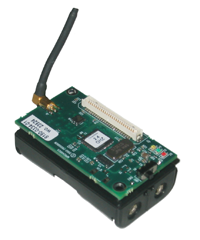
\includegraphics[scale=0.5]{images/micaz.png}
\caption{Crossbow MRP2600}
\label{fig:micaz}
\end{figure}

\subsection{Gateway Server}
The gateway server is a key component in the system. It is responsible for extracting Wi-Fi frames and forwarding them as Zigbee frames and vice versa. It is also responsible for receiving IPV4 packets and transforming them into IPV6 and vice versa. The gateway server has other functionalities such as the ability to receive sensor data from \gls{wsn} and forward them to the middle-ware. In case the link between the gateway server and the middle-ware is lost, the gateway server stores the received data in a temporary data store and communicate this data once the link is up again. This feature serves as a way to avoid losing sensory data.

\subsection{Middle-ware}
The middle-ware is a software component that is used to hide the heterogeneity of the system from external users. The middle-ware also provides automation mechanisms in order to control and reduce the energy consumption, but the main features are the ability to receive data, filter it, transform it and store it in a coherent fashion in order to use it smartly to reduce consumption. In addition, the middle-ware provides a set of web services that enable the clients to access all sorts of information such as the real-time consumption, daily, weekly and monthly consumption information inferred from the sensory data coming from the \gls{wsn}.

\subsection{Mobile Client}
The mobile client application is an application for Android phones that enable users to access the real-time consumption of their homes, and also to remotely control their appliance by turning On and Off any appliance linked to a mote in the \gls{wsn}. The mobile client when wanting to turn on or off some appliance sends a command directly to the mote responsible for controlling the mote and addresses the mote using its "virtual" \gls{ipv4} address that it does not own in really since it has an \gls{ipv6} address. This virtual \gls{ipv4} address is reserved for that mote and the translation is made at the gateway level.

\ Now that all components have been introduced, the data flow of the information is to be explained. As it was stated, any component in the system can communicate with any other independently of the data link layer technology or network layer technology.

\begin{figure}[htbp]
\centering
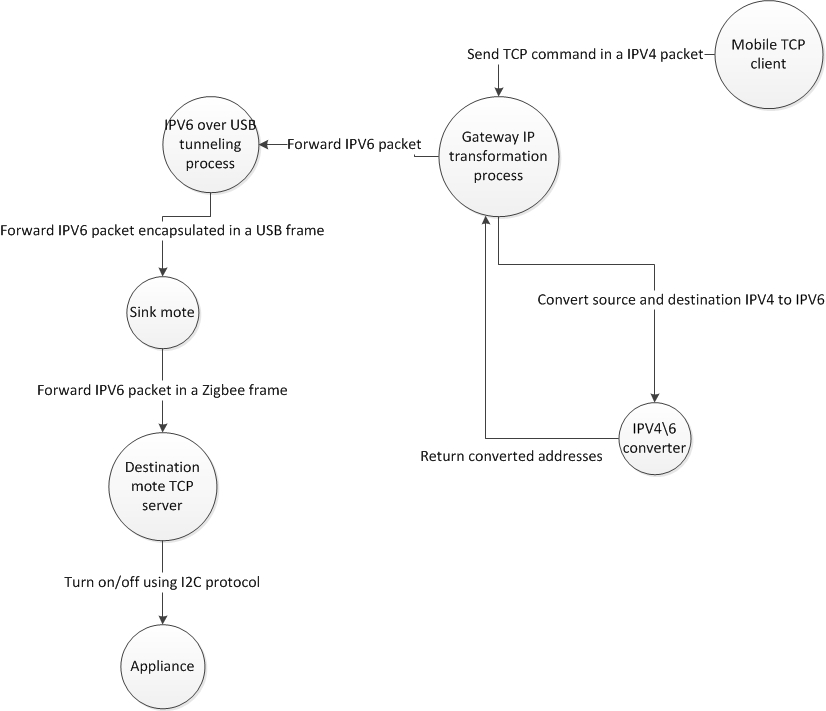
\includegraphics[height=110mm,width=90mm]{images/control_appliance_data_flow.jpg}
\caption{Data flow diagram for the mobile client sending on/off commands}
\label{fig:control_appliance}
\end{figure}

\
One of the main goals of this project is to build the two-way communication between the client and sensor nodes. To do so, the flow of data in both directions is depicted in figure \ref{fig:control_appliance} and figure \ref{fig:send_data}. The mobile client is connected to a Wi-Fi network that uses \gls{ipv4} whereas the \gls{wsn} uses \gls{ipv6}. Therefore, there should be a process that control and transforms the incoming and outgoing packets. The client starts by sending packet to the virtual \gls{ipv4} address of the mote. Afterwards, the gateway receives it, translates the virtual \gls{ipv4} address into the real \gls{ipv6} address of the mote by setting as source address the virtual \gls{ipv6} address of the mobile client. The new \gls{ipv6} packet is created carrying the payload coming from the original packet. This new \gls{ipv6} packet is forwarded to the wireless sensor network using an \gls{ipv6}-over-\gls{usb} tunnel that encapsulates the packet into a \gls{usb} frame and communicates it to the mote sink that extracts the \gls{ipv6} packet from the frame and encapsulates it into a Zigbee frame. Once the Zigbee frame arrives to the destination mote, the TCP datagram is extracted from the packet and passed to the TCP server of the mote that reads the message and executes it by turning on/off the appliance using I2C. 

\
The mote on the other hand sends periodically sensory data to the middle-ware, but again the communication passes through several steps which are depicted in figure 4.

\
The mote reads periodically sensory data from the sensor, transforms the data and communicates it. To send it, the mote client connects to a TCP server hosted at the gateway server. An \gls{ipv6} packet is encapsulated in a Zigbee frame that is forwarded to the mote sink that extracts the IPV6 packet, encapsulates it into a \gls{usb} frame and forwards it to the gateway that reads the TCP datagram. Once the sensory data is in the gateway, it communicates it to the middle-ware, and if the link is down, the sensory data is temporarily stored in a database hosted in the gateway. Once the link is up, all the stored data is sent to the middle-ware and cleared from the database.

\begin{figure}[htbp]
\centering
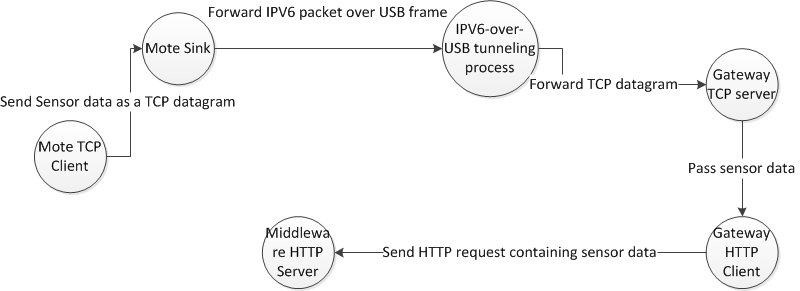
\includegraphics[scale=2.6]{images/send_sensor_data_data_flow.jpg}
\caption{Data flow diagram depicting the sending of the data}
\label{fig:send_data}
\end{figure}


\section{System Deployment}
To have a system that is capable of providing a two-way communication between any host and any mote in the \gls{wsn}, the following components have been built:
\begin{itemize}
\item Mote programming
\item Mote sink packet forwarding
\item Network gateway packet transformation
\item Network gateway sensor data server
\end{itemize}

\subsection{Mote Programming}
Each mote within the WSN network is equipped with a current transformer that is attached to data acquisition board through which data is read and transformed to the appropriate format and sent to the network host. In addition to this, the appliance is attached to the mote through the relay pins existing within the data acquisition board in the mote. In other words, the mote can control the electricity going to each mote and can allow it or block it. This means that one can control the appliance by using some of the functionalities provided by the mote. From the mote's perspective there are two parts that are implemented within its TinyOS program. A TCP server that is used to receive on/off requests in order to control the mote and a TCP client used to send sensor data.Once the program installed, an IPV6 address is passed to the installation routine in order to assign a static IPV6 address to the mote in which the program is cross-compiled and installed. The TCP server and TCP client work in parallel as each one's traffic is handled separately.

\subsubsection{TCP Server}
The TCP server is an important component in the mote's program. Any one willing to control the appliance must connect to the TCP server and send requests. As a mote may control more than one appliance, we then identify the appliance by a unique id and send a zero to turn off or one to turn on. Requests such as "1 1" means to turn on the appliance with id 1.
\subsubsection{TCP Client}
The TCP Client is an important component in the mote's program. It serves as mean to send sensor data to the gateway reliably. Once the mote is turned on, the client connects to a TCP server that is in the gateway, then the consumption data is sensed periodically (once per second) and sent to the TCP server who deals with the sensor data.

\subsection{Mote Sink Packet Forwarding}
The mote sink packet forwarding module is a special program installed within a mote that is equipped with a USB port that plays the role of a network interface card. The mote is attached to the gateway station and has the BLIP (Berkeley Low power IP stack Protocol) module within in. In addition it communicates with the gateway using USB protocol. In the gateway station, the network interface module is a sort of a IPV6 over USB tunnel which means that if an IPV6 packet packet is going to the sink, it is encapsulated within a USB frame and once it arrives to the mote, the IPV6 packet is extracted and forwarded to the destination mote holding that IPV6 address. The other way around is fairly similar, when a mote wants to send an IPV6 packet to the outside world, the mote creates the packet, sends it to the sink that forwards it by encapsulating it into a USB frame.

\subsection{IPv4/IPv6 Gateway}
This is a very important component in the system. The issue is the following. The WSN network supports only IPV6 while other components such as the middle-ware and the mobile client do not necessary have an IPV6 address, but we still want all the components to communicate independently of the IP technology to be used. To do so, we have created a network packet transformation program. This program basically converts IPV4 to IPV6 and vice versa. To do so, it assigns virtual IPV4 addresses to IPV6 address holders and and IPV6 address to IPV4 address holders. With such a program, each player in the network has both an IPV4 and an IPV6 but is aware of only the one that is assigned to him. The other "virtual" address is known only at the level of the program installed at the gateway station between the WSN and the outside world. 
\\
 The flow of information works as follow; when a station wants to send requests to a mote, it will send IPV4 packet holding the request to the mote but by addressing it using its virtual IPV4 address. This packet will be sniffed by this packet transformation program that will extract the TCP datagram from the ip packet, create a new IPV6 packet specifying the source address as the virtual address of the host and the destination as the address of the mote and then append the TCP datagram to the newly created packet and send it to the mote sink packet forwarding component that is seen by the gateway as a network interface card. This leads to a complicated issue that is to be handled and which is that the program should keep track of the request responses in order to forward them correctly to the destination. 
\\
To solve such a problem, an algorithm has been created whose sole role is to mechanically compute the IPV6 address of the host based on its IPV4 and vice versa. This algorithm is based on function whose primary quality is the fact that it is bijective which means any IPV4 address is mapped to one and only one IPV6 function and vice versa. So whenever a request is coming, the source and destination address will be converted using this algorithm and this will make avoid the whole request response tracking part.
\section{Findings}
The goal of this part is to measure to what extent is the system able to operate reliably by offering an acceptable level of performance. Two experiments were conducted to measure the system's performance. In the first experiment, the normal work of the system is simulated, where each mote reads sensory data every second and generates traffic in the \gls{wsn}. Our goal is to measure the delay and observe its variance as the traffic varies. The routing protocol in principle gives more priority to routing packets rather than processing them. Therefore, this priority must affect the network's delay. Table \ref{table:exp1} illustrates how the delay and jitter vary as more and more nearby motes are added to the network.
\begin{table}[htbp]
    \begin{tabular}{lll}
    \hline
    number of motes & Delay (ms) & Jitter (ms) \\\hline
    1               & 87.5         & 1.2         \\ 
    2               & 88.1         & 2.0         \\
    3               & 88.3        & 2.7         \\
    4               & 88.8         & 3.1         \\
    5               & 90.0         & 3.3         \\
    6               & 89.5         & 3.5         \\
    \end{tabular}
    \caption{Experiment 1 delay and jitter}
    \label{table:exp1}
\end{table}

\
It is clear that the average delay is not significantly affected by the number of motes in the network, but the jitter on the other hand is clearly affected by the number of motes in the network as it is depicted in figure \ref{fig:delay_jitter}. The delay is much more affected because there are time interval where the network is less busy and other intervals where the network becomes busier.
\begin{figure}[htbp]
\centering
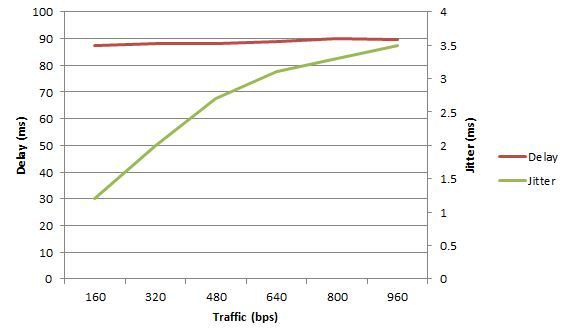
\includegraphics[scale=0.6]{images/delay_jitter.JPG}
\caption{Delay and jitter evolution by Traffic}
\label{fig:delay_jitter}
\end{figure}

The second experiment's goal is to measure the contribution of the Gateway Packet transformation process to the overall communication delay. The results gathered reflect the average delay and jitter computed over the elapsed time starting from the sniffing of the packet to the transformation and sending to the recipient. Table \ref{table:exp2} shows the result that was collected from this experiment as it was done on 200 packets that were sniffed and transformed by the system.

\begin{table}[htbp]
    \begin{tabular}{ll}
    \hline
    Delay ($\mu s$) & Jitter ($\mu s$) \\ \hline
    100        &  30        \\ 
    \end{tabular}
    \caption{Experiment 2 delay and jitter}
        \label{table:exp2}
\end{table}

\
The transformation process's elapsed time is measured in microseconds and from table \ref{table:exp2}, one can see that the average delay is on average 0.1 milliseconds whereas the jitter is around 0.03 milliseconds meaning that the process's time varies between a few microseconds to at most 150 microseconds. In addition, depending on the machine's load, the distribution of the delay frequency is shown the histogram depicted in figure \ref{fig:histogram}. From this figure one can conclude that the delay is normally distributed
\begin{figure}[htbp]
 \centering
 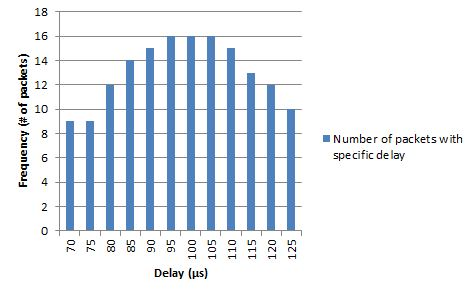
\includegraphics[scale=0.7]{images/histogram.JPG}
 \caption{Delay frequency histogram}
 \label{fig:histogram}
 \end{figure}
\section{Conclusion}
\glsreset{iot}\gls{iot} is the next revolution in computing. The test-bed presented in this paper shows how can Smart Grids by making use of numerous technologies such as \gls{iot} based \glspl{wsn}, \gls{6lowpan} in order to integrate it into \gls{iot} and benefit from it. The test-bed illustrates the two-way communication and also discusses the architecture of this system. 

\
The issues that were handled are mainly related to making the communication possible on a heterogeneous system where the data link layer and network standards used by different components of the system differs. The packet is transmitted from the an \gls{ipv4} network over Wi-Fi and moves to an \gls{ipv6} network over USB then to Zigbee. 

\
Smart Grids should benefit from the Internet of Things and will become one of the most important applications of \gls{iot} and therefore enable more efficient generation and consumption of data.

%Bibliography
\mbox{}
\nocite{*}
\bibliographystyle{IEEEtran} 
\bibliography{IEEEabrv,myrefs}
     

\end{document}


